\section{Introduction}
% problem description: semantic relatedness
Computing semantic relatedness(SR) between two elements(words, sentences,
texts etc.) is a fundamental task for many applications in Natural Language
Processing(NLP) such as lexicon induction(\cite{aaai/QadirMGL15}), Named 
Entity Disambiguation{\cite{acl/HanZ10}}, Keyword Extraction
(\cite{ijcai/ZhangFW13}) and Information Retrieval(\cite{acl/GurevychMZ07}). 
Additionaly, computing semantic relatedness contributes other applications, 
for example, opinion spam problem (\cite{www/SandulescuE15}) and so on(+some example). 
In this paper we focus on computing semantic relatedness between two 
words in knowledge graph with neural network.

It has long been thought that when human measure the relatedness between
a pair of words, a deeper reasoning is triggered to compare the concepts
behind the words. Many traditional studies on semantic relatedness
utilize different data sources to compute semantic relatedness. There are
i) \emph{the large corpora}, such as wikipedia(\cite{ijcai/GabrilovichM07}), 
ii) \emph{the lexical databases}, such as WordNet(\cite{acl/Pucher07}) or Wikithionary(\cite{aaai/ZeschMG08}), 
iii) \emph{the knowledge graph}, such as DBpedia(\cite{aaai/NavigliP12}) or BabelNet(\cite{aaai/NavigliP12}).
With the development knowledge representation, computing semantic relatedness using
knowledge-rich resouce is a well-explored line of research. It is known to all that
knowledge graph contains both syntactic and semantic information which are 
richer than lexical databases, and more sturctured knowledge than the large corpora.
On the account of advantages of knowledge graph, we use it as background 
knowledge to computing semantic relatedness.

% Knowledge graph can be accessed with powerful query language Sparql in RDF graph.
% As for the methods build on the data soruce, the recent word embedding 
% learning approaches demonstrate their abilities
% to capture syntactic and semantic information, and outperform the
% lexicon-based methods\cite{acl/Pucher07}. 
% Knowledge Graph, as a semantic graph, stores
% vast amount of sturctured knowledge. 

\begin{figure*}
    \centering
    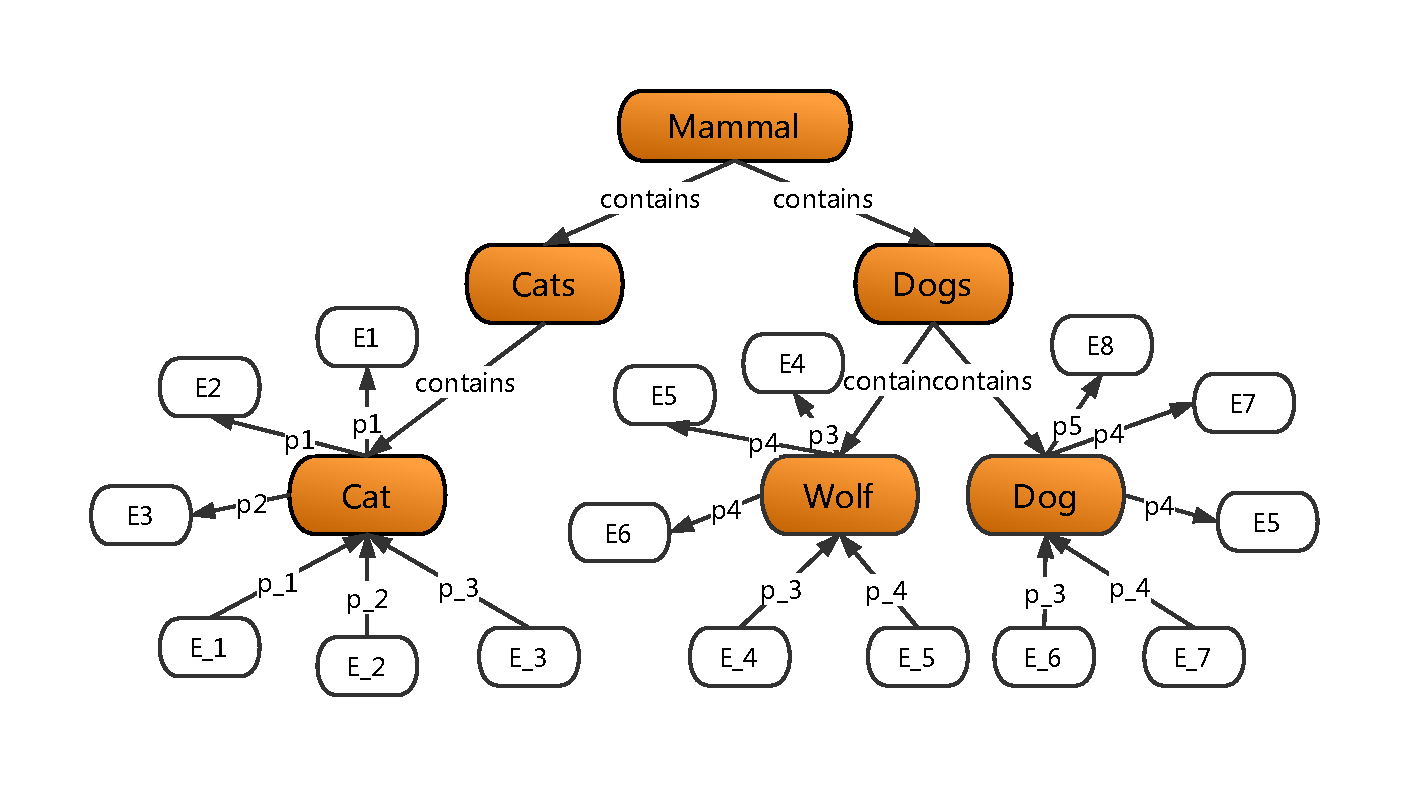
\includegraphics[width=1.0\textwidth]{pic/weak1.pdf}\\
    \caption{Subgraph example in knowledge graph}
    \label{weak1}
\end{figure*}

Recently, there are some researchs have attached importance to measure semantic relatedness
in knowledge graph\cite{aaai/Pirro12, aaai/NavigliP12, acl/IacobacciPN15}. 
\cite{acl/IacobacciPN15} leverage entity linking to annotate the dump of wikipedia. Based on this,
the sense-annotated corpus is generated. Then the author using word2vec to
train the sense-annotated corpus getting distributed representation of different 
word sense. This step still need a significant preprocessing and data transformation effort. 
As we can see this approache computing semantic relatedness on account of large corpora.
The author just put the knowledge graph on the position of support. 
\cite{aaai/NavigliP12} presents a knowledge-rich approach to computing multilingual semantic
relatedness which exploits the joint contribution of different languages. Given a pair of words 
in two languages they use BabelNet to collect their translations, compute semantic
graphs in a variety of languages, and then combine the empirical evidence from these 
different languages by intersecting their respective graphs.
\cite{aaai/Pirro12} propose an approache exploiting the graph nature of RDF and SPARQL query
Language to access knowledge graph. It not only obtains the comparable
result with the state-of-art at that moment, but also avoids the burden
of preprocessing and data transformation.




Though \cite{aaai/Pirro12} avoids a significant preprocessing and data
transformation effort, which develops it scalability when adopting a
different source of knowledge graph, they miss some factors which
have contributed to semantic relatedness measure. Firstly, given two words
as input, the first step is to find corresponding entities in knowledge
graph. Obviously, there are not only one entity in knowledge graph for a single
word. For a input word \emph{car}, for example, we will get \emph{:Automobile} and
\emph{:Auto\underline{\hspace{0.5em}}Racing} and so on. \cite{aaai/Pirro12} lose
sight of the informativeness of the other entities, while they just
consider the entity with the highest rank. Secondly, \cite{aaai/Pirro12} misses
some informativeness of \emph{predicates} as their stategy takes
the predicates into account exclusively based on the TFIDF. This
method ignore the function of \emph{objects} in a semantic triple.
As show in Fig\ref{weak1}, subgraph contains \emph{Dogs} and \emph{Cats} extracted from
knowledge. We simplify the sepcific features of entities to concise symbol. 
We can see that entities in knowledge graph such as \emph{Cat} can play the role 
of both \emph{Object} and \emph{Subject} in a pattern of triple, which means a predicate 
\emph{p$_i$} may be used as an incoming or outgoing predicate w.r.t a entity
\emph{E$_i$}. The relatedness space for a entity \emph{E$_i$} is modelled a 
k-dimensional weighted vector \emph{V$_i$}, where each dimension represents
the informativeness of a specific predicate\cite{BudanitskyH06}. For example, the weighted
vector for \emph{Cat} is 
[\emph{v$_{p1}$}, \emph{v$_{p2}$}, \emph{v$_{p1}$$^,$}, \emph{v$_{p2}$$^,$}, \emph{v$_{p1}$$^,$}]. 
Obviously, while the author was considering the informativeness of a specific 
predicate, ignore the the implications contained in the connected entities(e.g.
\emph{E$_1$}, \emph{E$_2$}). The author do not distinguish the different 
objects w.r.t a specific predicate. In order to improve the perfomance the computing
of semantic relatedness based on knowledge graph, we propose a model to touch 
the target. Our model is threefold.

1. For given word pairs, the first job is to query
the corresponding entities. In order to use the
translating embedding for training the dataset, we
also need to construct a graph contains all realted
entities and relations between the corresponding
entity pairs.

2. We use translating embedding for knowledge
graph instead of Word2vec to train the subgraph
extracted from the knowledge graph. Then we can
get a distributional representation(vector) for each
entities and predicates. 

3. When we take as inputs a word, we can get several 
corresponding entities. Inspired by \cite{acl/IacobacciPN15}, we use 
a approache to combine the relatedness score resulting from the
entity as the finnal semantic relatedness score in knowledge graph.

This paper is organized as below. 